\section{Profil wykonawcy i komentarze}

Dla klientów bardzo ważna jest możliwość przeglądania informacji dotyczących wykonawców. Na ich podstawie mogą bowiem opierać podejmowane przez siebie decyzje. Wykonawcy również potrzebują podobnej możliwości, by móc zobaczyć informacje dotyczące siebie samych. Z tych powodów funkcjonalność przeglądania profilu wykonawcy i komentarzy została dodana do obu aplikacji.

\begin{figure}[ht]
  \captionsetup[subfigure]{justification=centering}
  \centering
  \begin{subfigure}[t]{0.32\textwidth}
    \centering
    \fbox{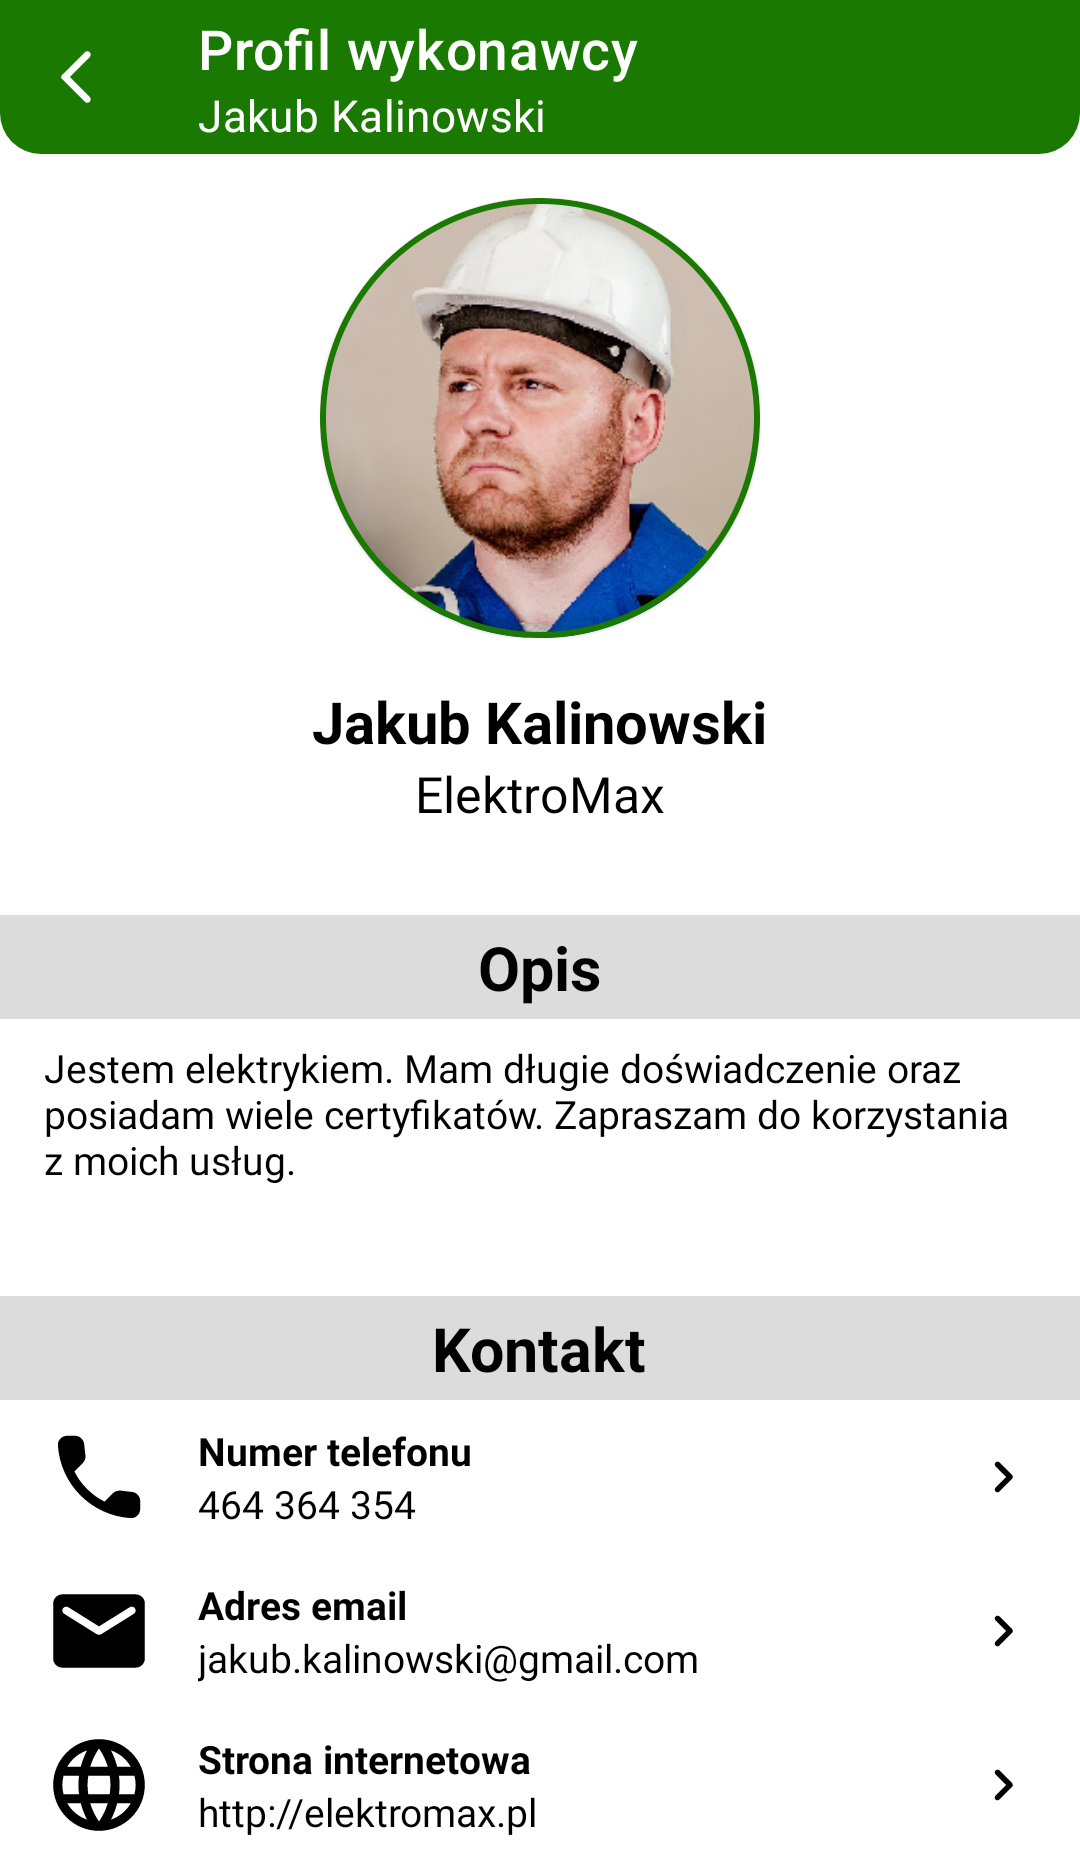
\includegraphics[width=0.97\linewidth]{screens/profile_1.png}}
  \end{subfigure}
  \begin{subfigure}[t]{0.32\textwidth}
    \centering
    \fbox{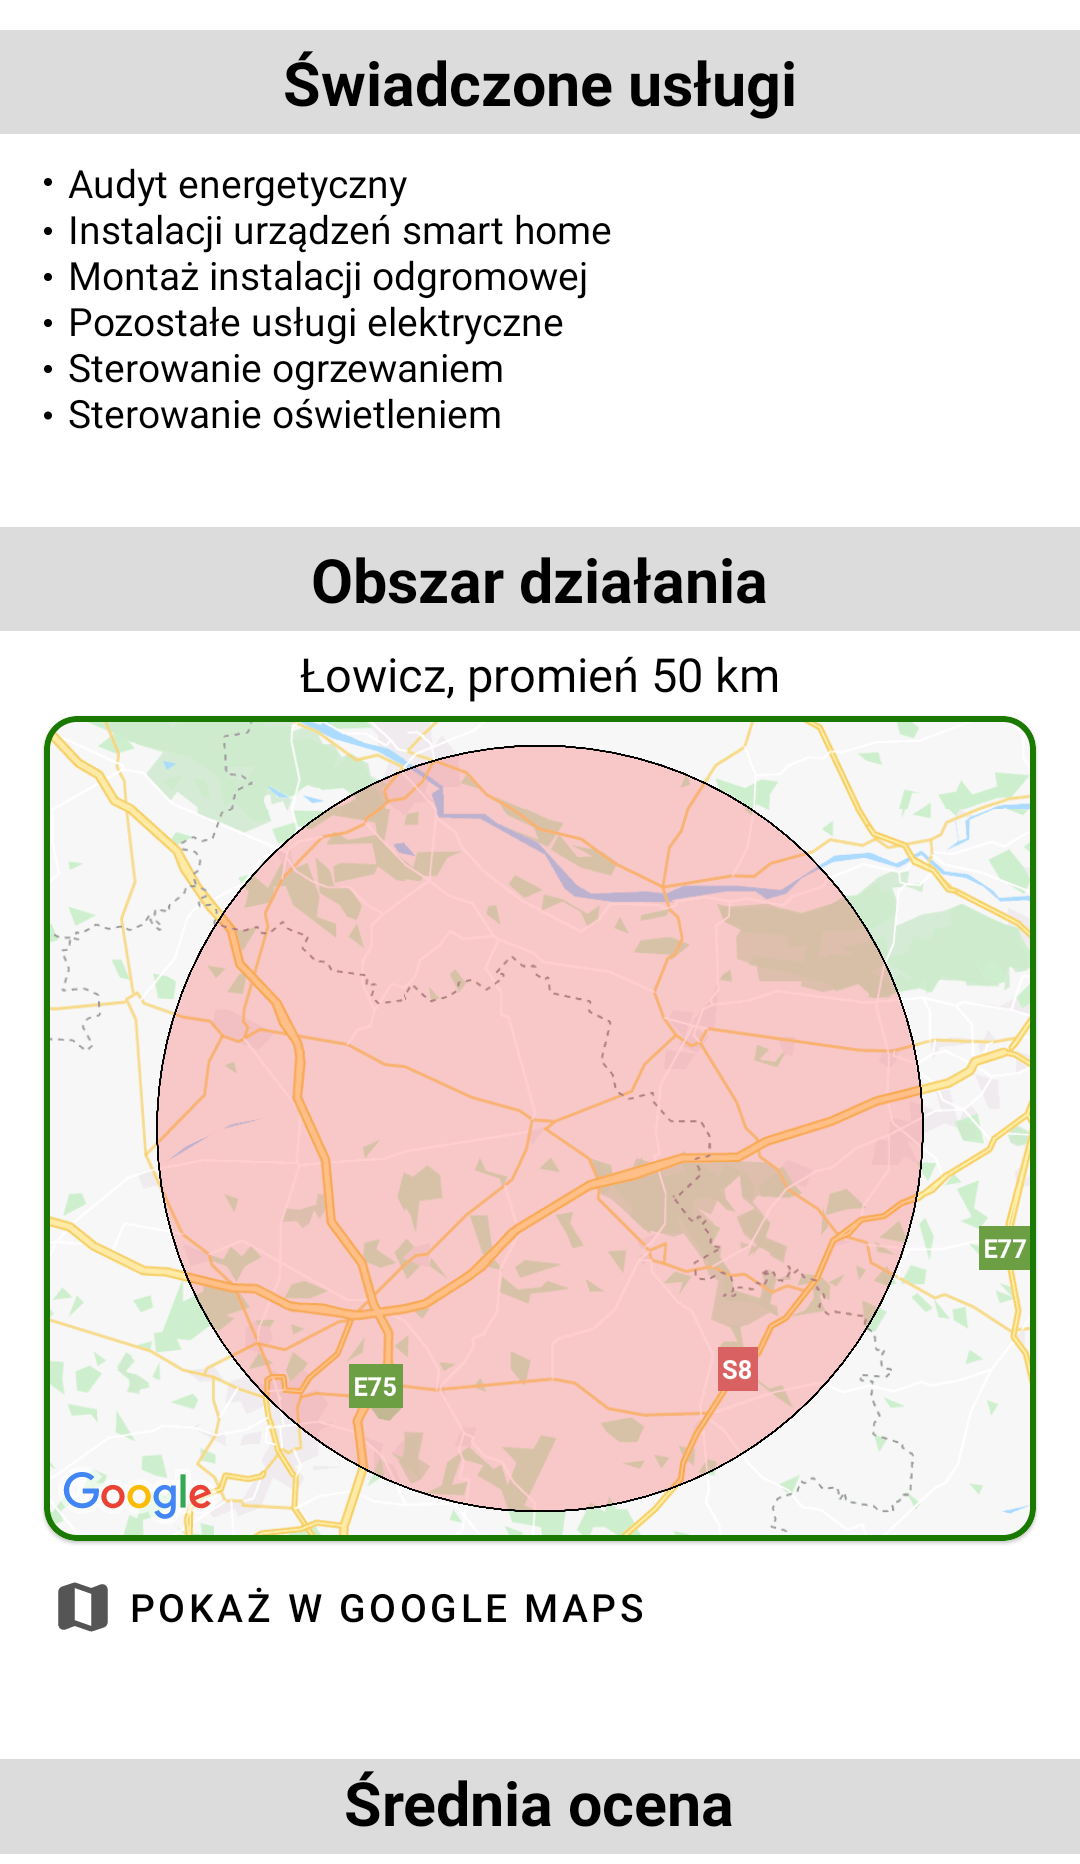
\includegraphics[width=0.97\linewidth]{screens/profile_2.png}}
  \end{subfigure}
  \begin{subfigure}[t]{0.32\textwidth}
    \centering
    \fbox{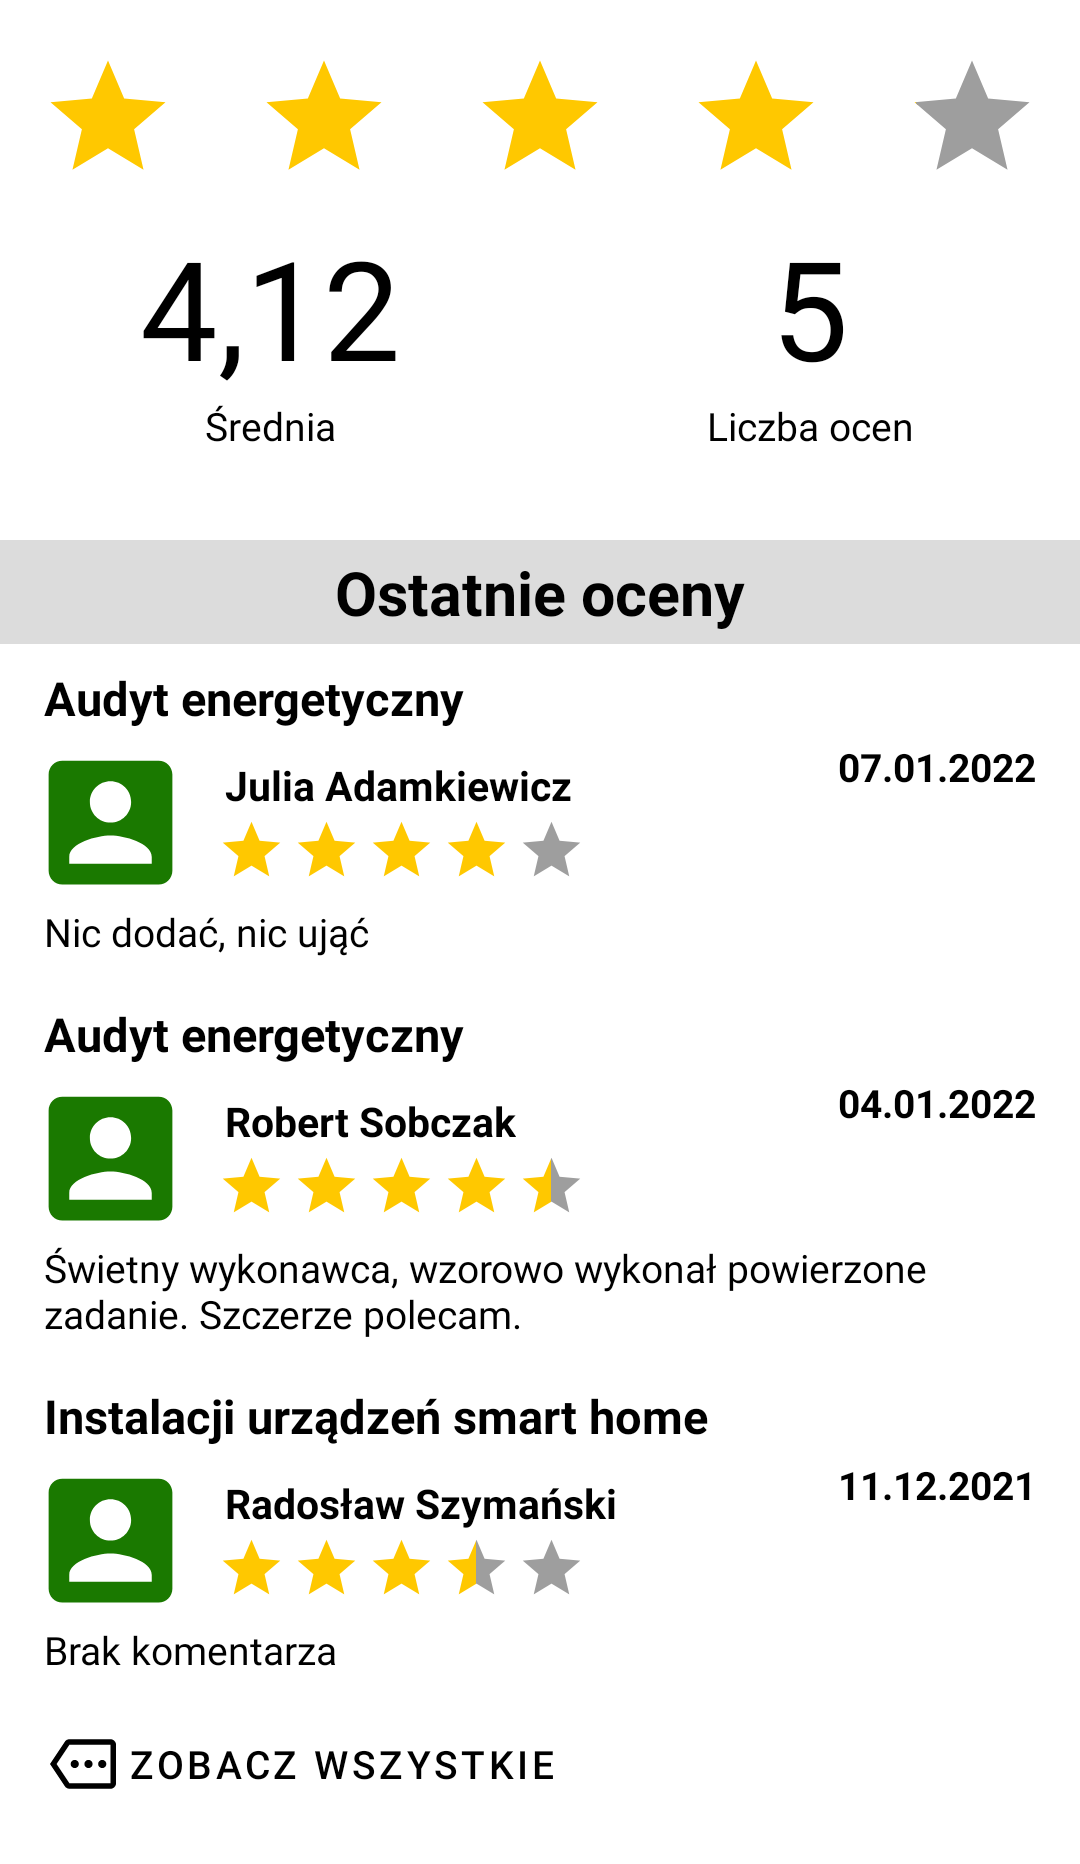
\includegraphics[width=0.97\linewidth]{screens/profile_3.png}}
  \end{subfigure}
  \caption[Ekran profilu wykonawcy]{Ekran profilu wykonawcy w aplikacji dla klientów}
  \label{fig:profile}
\end{figure}

Okazuje się, że przeprowadzone zostały dokładne badania dotyczące strategii podejmowania decyzji przez klientów podczas zakupów online. W jednym z artykułów \cite{ratings-presentation} stwierdza się, że pomimo tego, iż mają oni zwykle dostępnych wiele źródeł informacji, to często szukają możliwości uproszczenia swoich decyzji i wyciągnięcia sedna. Z tego powodu postanowiono umieścić w widocznym miejscu średnią ocenę wykonawcy, która jest dobrym wskaźnikiem do tego celu. Można to zobaczyć na rysunku \ref{fig:profile}.

Na ekranie profilu wykonawcy postanowiono umieścić jedynie trzy ostatnio dodane komentarze. W celu zobaczenia pełnej listy konieczne jest przejście do oddzielnego ekranu, na którym się one znajdują. Ponieważ niektóre mogą być długie, postanowiono je przyciąć do długości trzech linii. Aby zobaczyć wówczas całą treść należy wybrać konkretny komentarz. Odpowiednie widoki przedstawiono na rysunku \ref{fig:ratings}.

\begin{figure}[ht]
  \captionsetup[subfigure]{justification=centering}
  \centering
  \begin{subfigure}[t]{0.32\textwidth}
    \centering
    \fbox{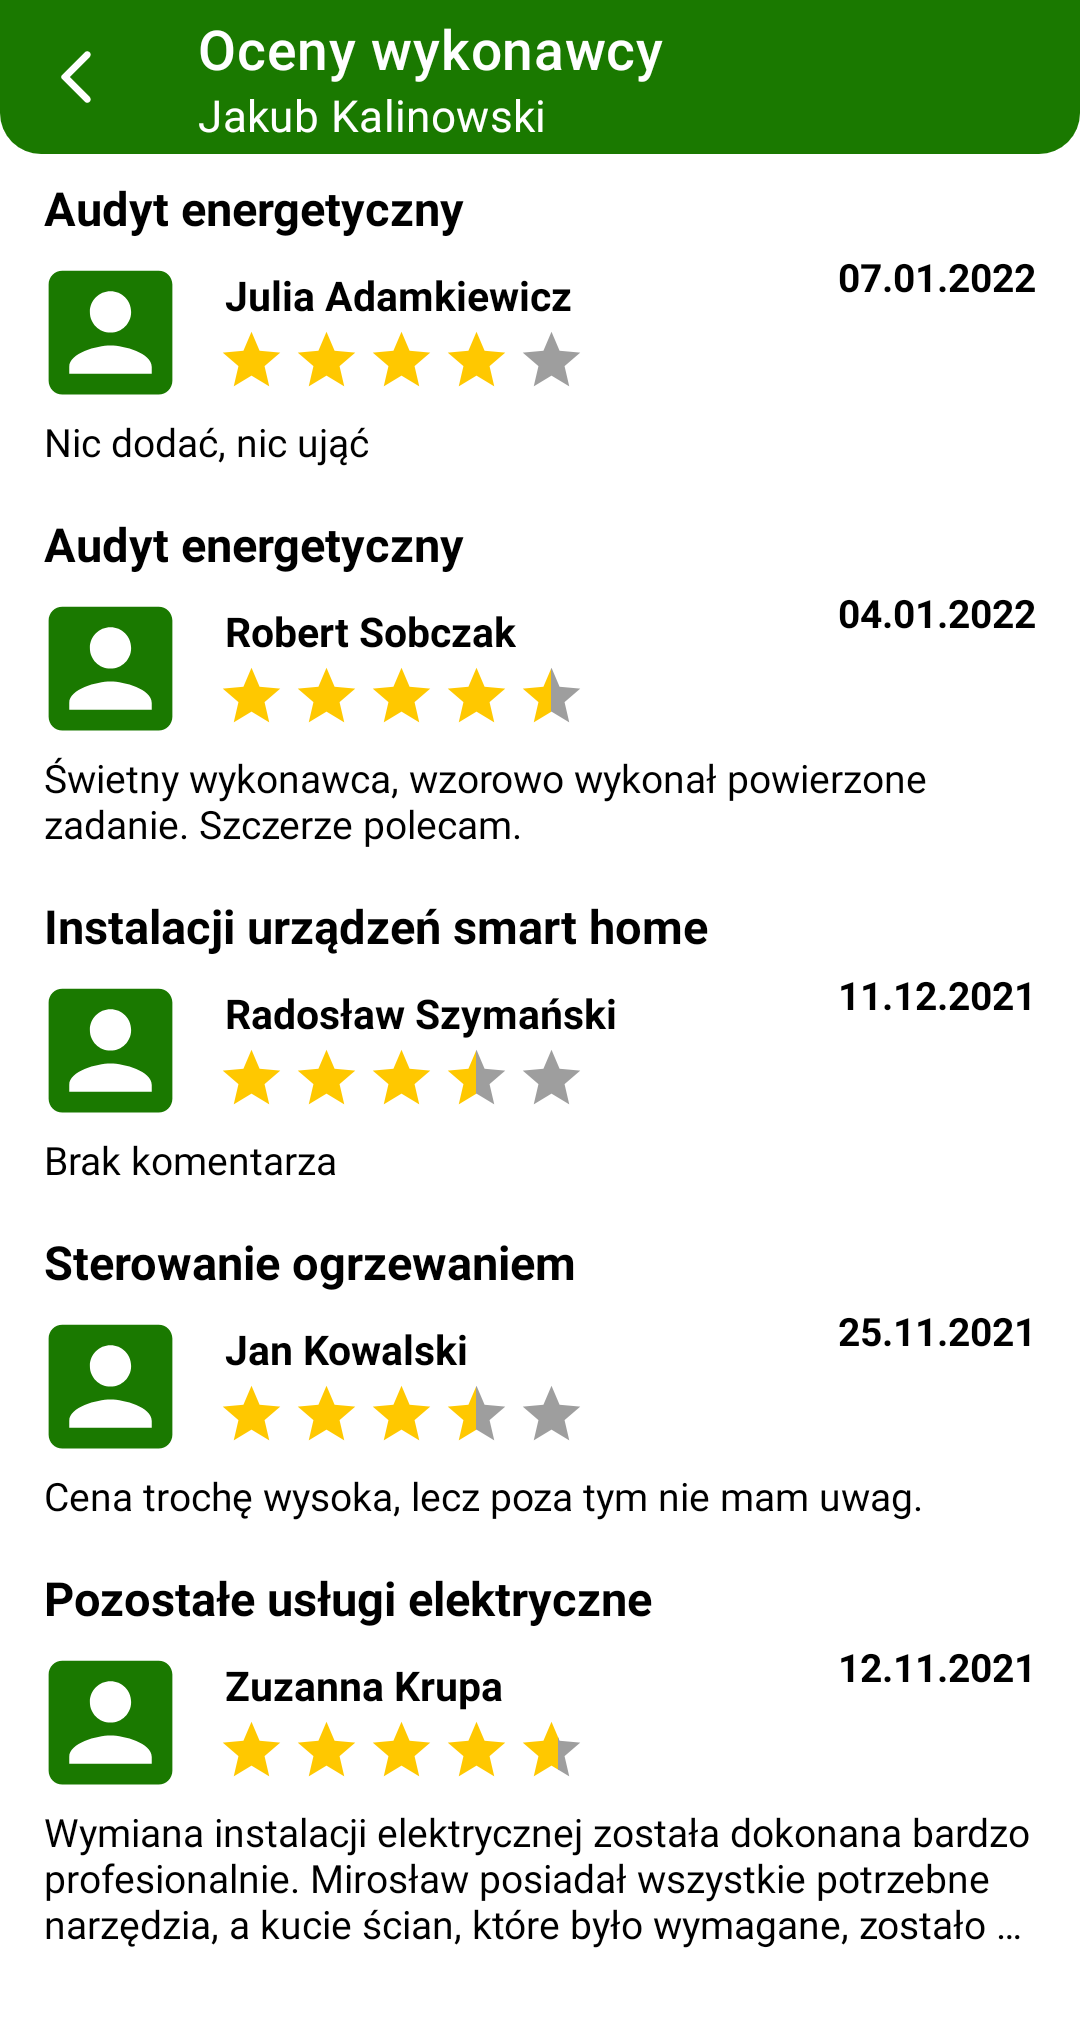
\includegraphics[width=0.97\linewidth]{screens/ratings.png}}
    \caption{Ekran wszystkich komentarzy}
  \end{subfigure}
  \begin{subfigure}[t]{0.32\textwidth}
    \centering
    \fbox{
\includegraphics[width=0.97\linewidth]{screens/rating.png}}
    \caption{Ekran wybranego komentarza}
  \end{subfigure}
  \caption{Ekrany komentarzy}
  \label{fig:ratings}
\end{figure}
